\chapter{Previous Results}
\label{chapter:previous}

\section{Observations and properties of the \Z boson}
The first indirect experimental evidence for the \Z boson was first observed at the
Gargamelle detector at CERN~\cite{Hasert:1973uq} in 1973. The experiment
consisted of passing a neutrino beam through a liquid bubble chamber and looking
for evidence of neutral currents in the form of electron-neutrino scattering:

\begin{equation*}
\overline{\nu}_{\mu} + e^- \rightarrow \overline{\nu}_{\mu} +  e^- \newline
\end{equation*}
\begin{equation*}
\nu_{\mu} +  e^- \rightarrow \nu_{\mu} +  e^-
\end{equation*}
Of the 735,000 pictures analyzed, one was characteristic of a neutral current
interaction, and is regarded as the first experimental evidence of the \Z boson.

The first direct evidence of the particle came almost a full 10 years later, in
1983, at CERN's Super Proton Synchrotron (SPS). The UA1 experiment observed four
events indicative of a $\Z\rightarrow e^+e^-$ decay and one $\Z\rightarrow
\mu^+\mu^-$ event, with invariant masses consistent with the SM prediction of
91.2 GeV\cite{UA1:Zobs}. The UA2 experiment corroborated the discovery soon
after.

Although the experiments at the SPS were able to provide the first evidence of
the \Z boson, it was not until the clean collisions recorded by the experiments
at CERN's Large Electron-Positron (LEP) collider that accurate measurements of
the boson's properties could be made in 1990. The energy of the collider, combined with
the clean environment of electron-positron collisions, made the experiments at
LEP a veritable factor of weak bosons. When coupled with data from the SLAC
Large Detector (SLD) at the Stanford Linear Collider, the electroweak sector was
fleshed out in intricate detail.  Unparalleled measurements of mass, total and
partial decay widths, coupling constants, and searches for new decay modes and
anomalous coupling modes were conducted at the LEP and SLAC experiments. The
results were superb validations of the Standard Model predictions, with mass
measurement and widths measured with per-mil accuracy.~\cite{lepSLD:zPhys}:

\begin{equation*}
    m_Z = 91.91875 \pm 0.0021 GeV \\
\end{equation*}
\begin{equation*}
    \Gamma_Z = 2.4952 \pm 0.0023 GeV
\end{equation*}
\begin{equation*}
    sin^2 \theta_W = 0.23153 \pm 0.00016
\end{equation*}

Experiments the Tevatron (especially during its Run II phase from 2001 to 2011)
repeated these measurements within the context of 1.96~GeV $p\overline p$
collisions, with cross-section and weak-mixing angles fully consistent with
Standard Model expectations~\cite{cdf:weakMixingAngle, d0:weakMixingAngle}


\section{Diboson Production}
ZZ diboson events were first observable at the LEP experiments when the $e^+e^-$
center of mass energy exceeded the ZZ kinematic threshold. ALEPH, DELPHI, L3,
and OPAL reported ZZ production cross sections fully consistent with Standard
Model Expectations~\cite{ALEPH:zz, DELPHI:zz, L3:zz, OPAL:zz}.

Because the $ZZ\rightarrow4\ell$ final state has such a low branching ratio,
previous experiments have observed a statistically limited sample of $4\ell$
events.  The latest Tevatron results include only a handful in each
detector~\cite{CDF:zz, D0:zz}. %, as evidenced in Figure~\ref{fig:tevatronZZ}.


%\begin{figure}[h]
%\centering
%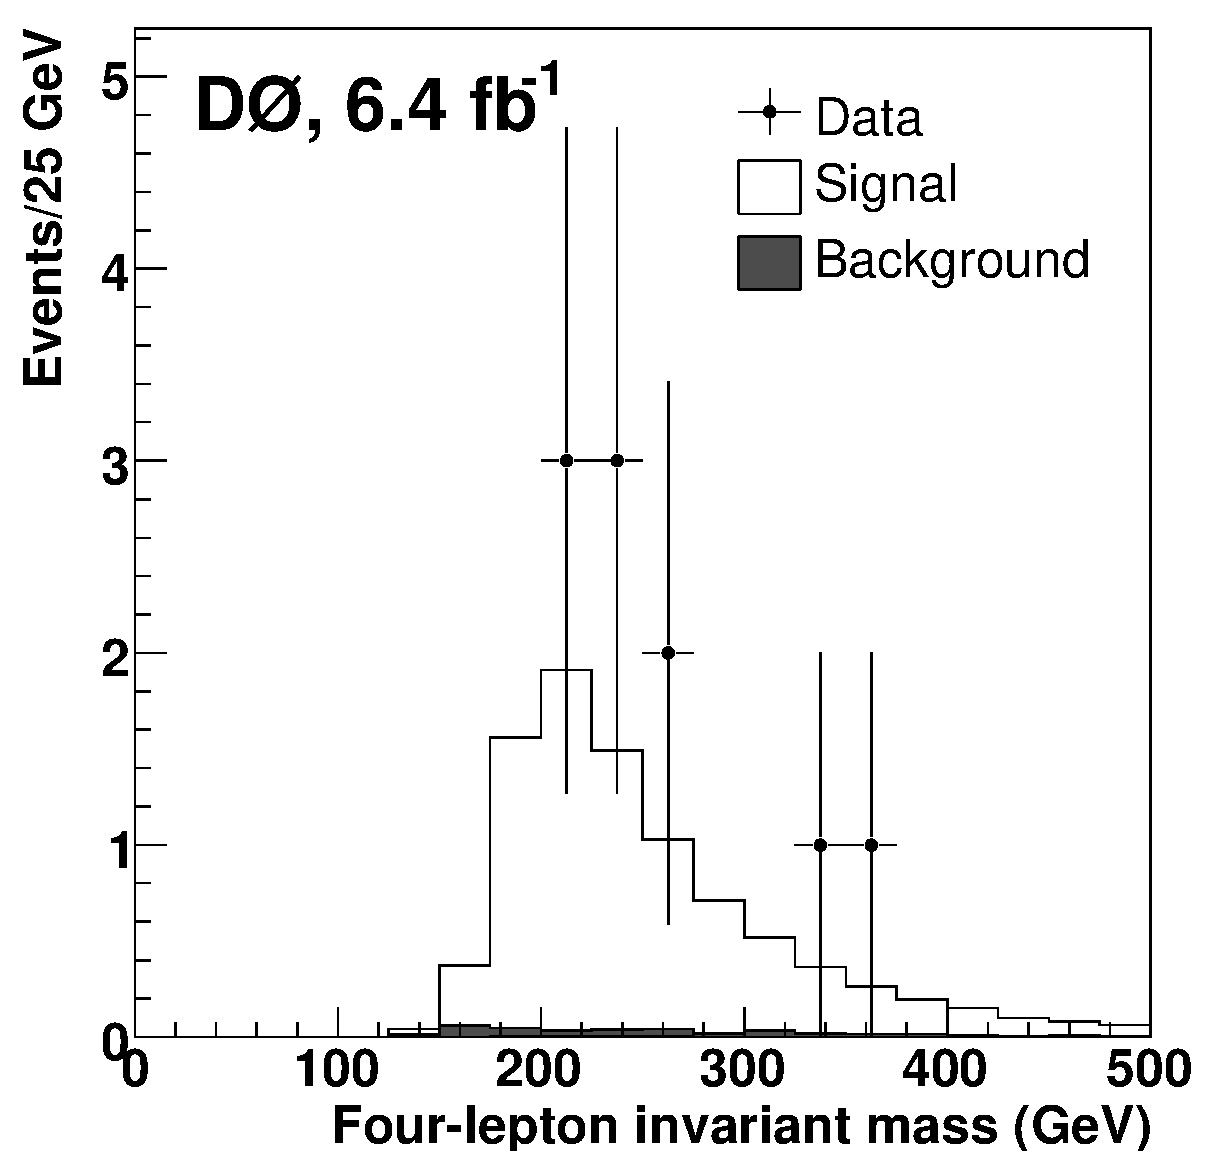
\includegraphics[width=0.45\textwidth]{d0_4lmass} %from http://www-cdf.fnal.gov/physics/ewk/2013/ZZ_97fb/ZZ4l.html
%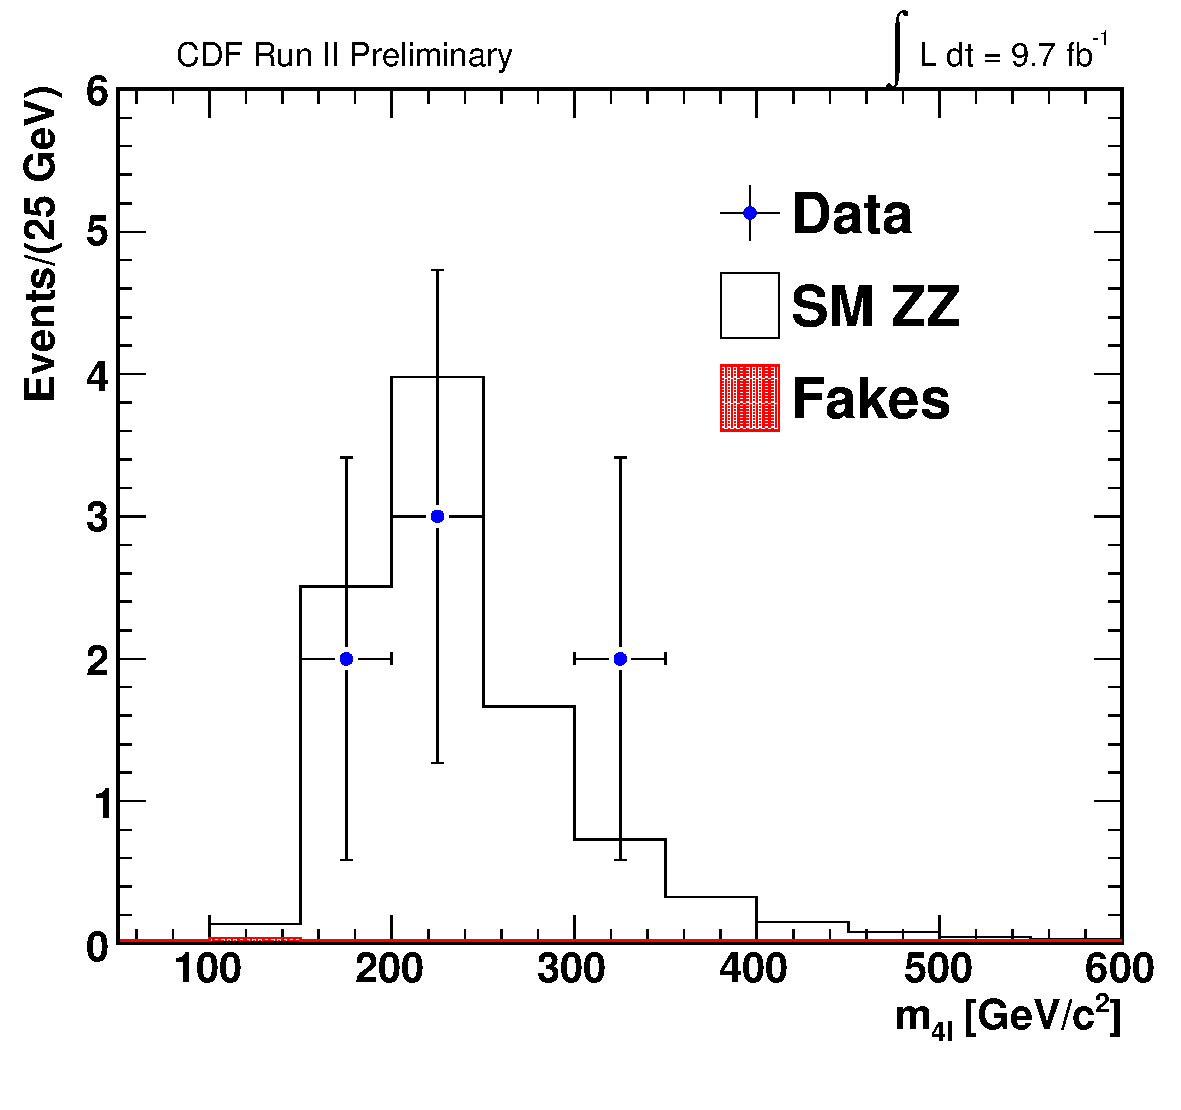
\includegraphics[width=0.45\textwidth]{cdf_4lmass} %from http://www-d0.fnal.gov/Run2Physics/WWW/results/final/EW/E11A/
%\caption[Tevatron observations of ZZ$\rightarrow$4l events.]{Observed four-lepton invariant mass for the Tevatron experiments. The
%data represent 6.4 \fbinv and 9.7 \fbinv of 1.96 TeV $p\overline p$ collisions
%at D0 and CDF (left and right, respectively).}
%\label{fig:tevatronZZ}
%\end{figure}

\section{Higgs Limits}
Experiments have been keen to observe the Higgs boson since its inception in the
1950s \cite{PhysRevLett.13.508, PhysRevLett.13.321, PhysRevLett.13.585}. While
the evidence remained elusive until the summer of 2012, the regions of possible
Higgs mass were constrained to ever-tighter regions of phase space.

After running from 1989-2000, the experiments at the Large Electron-Positron
(LEP) at CERN combined their direct searches to set a lower bound on the Higgs
Mass of 114.4 GeV~\cite{LEP:higgsLim} at 95\% Confidence level (CL).

Using the combined data from the LEP, SLC, and Tevatron experiments, a combined
fit to electroweak parameters was able to set an upper mass limit of 158
GeV~\cite{Grunewald:1313716}. %explain more?

Direct searches at the Tevatron ruled out $100 < m_H < 103$~GeV and
$147 < m_H < 180$~GeV at the 95\% confidence level, while reporting a broad
access of with a 2.9$\sigma$ significance~\cite{fnal:higgs}.

\section{Higgs Searches at the Large Hadron Collider}
The LHC was built with the Higgs boson in mind. As mentioned
in~\ref{sec:protonCollisions}, the proton-proton collisions provide an enhanced
rate of Higgs production, with expectations of either discovering the Higgs
boson at any mass, should it exist, or ruling out the mechanism entirely.

, with capability to produce Higgs boson, if it exists,
in sufficient quantity for any mass enabling a discovery or excluding the
mechanism itself.

Data taken at 7 TeV collision energy in the first two years of running left only
a small section of mass space for the Higgs boson. The first 5
\fbinv of data collected at 7~TeV allowed both the ATLAS and CMS experiments to carve out
a large portion of mass exclusion.  ATLAS ruled out (at 95\% CL) the masses
between 111.4-116.6, 119.4-122.1, and 129.2-541 GeV. CMS excluded from 127-600
GeV. By the time that the LHC was turned on again in 2012 (at 8 TeV
center-of-mass energy), only masses between 122.1 and 127 GeV had not been ruled
out at the 95\% CL. By the middle of the summer of 2012, the experiments had
gathered an additional 5 \fbinv at the higher energy and were able to announce,
on July 4, statistically significant evidence of a new
boson~\cite{cms:HiggsObs, atlas:HiggsObs}. Running through the end of 2012
produced another 15 \fbinv for the experiments, allowing each to begin to
characterize the particle. By all standards, the discovery does indeed look to
be the revered Higgs boson~\cite{ATLAS:higgsProperties, CMS:higgsProperties}.

%table with all limits

\section{Searches for neutral triple gauge couplings}
Searches for anomalous neutral triple gauge couplings have been performed at
LEP2~\cite{ALEPH, DELPHI, OPAL, LEPWG, L3}, the Tevatron~\cite{D0, CDF}, and
the LHC~\cite{ATLAS, ATLAS2, CMS}. Since no direct evidence has been
observed, all results are quoted as upper limits. The most stringent limits to 
date were set by the author and the CMS collaboration \cite{CMS}. The
limits on each of the couplings are summarized in~\ref{tab:atgcPrevLimits}.

\begin{table}[htbp]
\footnotesize
\centering
\setlength{\tabcolsep}{5pt}
\begin{tabular}{|c|c|c|c|c|l|}
\hline
Experiment & $f_4^Z$ & $f_4^\gamma$ & $f_5^Z$ & $f_5^\gamma$ &  Comments
\\
\hline
\hline
ALEPH~\cite{ALEPH}           & [-0.60;0.61] & [-0.40;0.36] & [-1.22;1.10] & [-0.81;0.79] &
2D fit results\\
\hline
DELPHI~\cite{DELPHI}          & [-0.40;0.42] & [-0.23;0.25] & [-0.38;0.62] & [-0.52;0.58] &
 \\
\hline
L3~\cite{L3}              & [-1.9;1.9] & [-1.1;1.2] & [-5.0;4.5] & [-3.0;2.9] 
& $\surd{s} = 189$ GeV\\
\hline
OPAL~\cite{OPAL}         & [-0.45;0.58] & [-0.32;0.33] & [-0.94;0.25] & [-0.71;0.59] & \\
\hline
LEP WG~\cite{LEPWG}               & [-0.30;0.30] & [-0.17;0.19] & [-0.34;0.38] & [-0.32;0.36]
& LEP combination\\
\hline
\hline
CDF~\cite{CDF}         & [-0.12;0.12] & [-0.10;0.10] & [-0.13;0.12] & [-0.11;0.11] &
$\Lambda$=1.2 TeV \\
\hline
D0~\cite{D0}          & [-0.28;0.28] & [-0.26;0.26] & [-0.31;0.29] & [-0.20;0.28] &
\begin{tabular}{@{}c@{}} $\sim 1$ \fbinv, \\ $\Lambda$=1.2 TeV \end{tabular} \\
\hline
\hline
ATLAS~\cite{ATLAS}           & [-0.12;0.12] & [-0.15;0.15] & [-0.13;0.13] & [-0.13;0.13] &
\begin{tabular}{@{}c@{}} $\sim 1$ \fbinv, \\$\Lambda$=2 TeV \end{tabular}\\
\hline
ATLAS~\cite{ATLAS}           & [-0.07;0.07] & [-0.08;0.08] & [-0.07;0.07] & [-0.08;0.08] &
\begin{tabular}{@{}c@{}} $\sim 1$ \fbinv,\\ $\Lambda$=inf \end{tabular}\\
\hline
ATLAS~\cite{ATLAS2}          & [-0.019,0.019] & [-0.022,0.023] & [-0.020,0.019]
& [-0.023,0.023] &
\begin{tabular}{@{}c@{}} 4.6 \fbinv,\\ $\Lambda$=3~TeV \end{tabular}\\
\hline
ATLAS~\cite{ATLAS2}          & [-0.013,0.013] & [-0.015,0.015] & [-0.013,0.013]
& [-0.016,0.015] &
\begin{tabular}{@{}c@{}} 4.6 \fbinv,\\ $\Lambda$=inf \end{tabular}\\
\hline
CMS~\cite{CMS}           & [-0.011;0.012] & [-0.013,0.015] & [-0.012,0.012] &
[-0.014,0.014] &
\begin{tabular}{@{}c@{}} $\sim 5$ \fbinv, \\$\Lambda$=inf \end{tabular}\\
\hline
\end{tabular}
\vspace{0.5cm}
\caption[Summary of existing 95\% C.L  for neutral aTGCs.]{Summary of existing 95\% C.L. intervals for the neutral aTGC $f_4^Z$,
$f_4^\gamma$, $f_5^Z$ and $f_5^\gamma$.
}
\label{tab:atgcPrevLimits}
\end{table}
